Bevor es mit der eigentlichen Bearbeitung des Themas in dieser Arbeit los geht, folgen an dieser Stelle zunächst einmal Erläuterungen einiger Grundbegriffe und Technologien. Diese werden im weiteren Verlauf der Thesis genutzt und sollen deshalb für ein besseres Verständnis schon einmal vorab eingeführt werden, falls diese noch nicht bekannt sind.

\subsection{Traveling Salesman Problem (TSP)}
\label{sec:grundlagen_tsp}
\todo{NP-schwer erwähnen?!}

Das \textit{Traveling Salesman Problem}, im deutschen auch bekannt als das \textit{Problem des Handlungsreisenden}, ist ein schon sehr altes Problem der theoretischen Informatik. Es handelt sich dabei um ein kombinatorisches Optimierungsproblem. Die Problemstellung selbst ist dabei sehr einfach erklärt: Ein Handlungsreisender möchte eine Menge von Stationen mit einer möglichst kurzen Reisestrecke besuchen. Jede Station soll dabei genau einmal besucht werden und die erste Station ist gleich der letzten, sodass ein Kreis entsteht. Ziel der Optimierung ist es also, die bestmögliche Reihenfolge der zu besuchenden Orte zu finden (ein beispielhaftes Problem und dessen Lösung ist in Abb. \ref{fig:tsp_deutschland} dargestellt). \cite{travelingSalesman}

\begin{figure}[H]
    \centering
    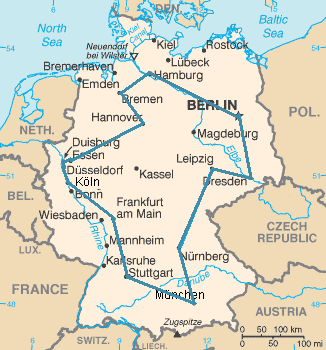
\includegraphics[width=0.5\textwidth]{images/TSP_Deutschland_3.png}
    \caption{TSP Beispiel - Beste Reiseroute durch die 15 größten Städte in Deutschland \cite{tspDeutschland}}
    \label{fig:tsp_deutschland}
\end{figure}

Modellieren lässt sich das Problem als Graph, bei dem die Knoten den Städten entsprechen und Kanten mit Gewichtungen den Aufwand der Reise zwischen diesen Städten darstellen. Das Problem der optimalen Wegfindung innerhalb eines Graphen lässt sich aber auch auf eine Vielzahl von anderen Problemen übertragen. Es hat somit eine große Bedeutung innerhalb der Informatik. Das möglichst schnelle Finden einer möglichst guten Lösung kann viele Probleme lösen, weshalb es bis heute Bestrebungen zur Suche nach guten Lösungsverfahren gibt. \cite{travelingSalesman} 

Das TSP ist allerdings ein sehr komplexes Problem, es gibt keine bekannte und effiziente Lösung dafür. Die Schwierigkeit ist, dass die Zahl der Kanten exponentiell mit der Zahl der Knoten n steigt. Sie folgt der Formel $n(n-1)/2$ \cite{graphenEckenKanten}. Ein vollständiger Graph aus vier Knoten hat so beispielsweise sechs Kanten, während es für fünf Knoten schon zehn Kanten und für zehn Knoten braucht es bereits 45 Kanten. Lösungsverfahren teilen sich in exakte und heuristische Verfahren auf. Exakte Verfahren gehen meist alle Wege oder zumindest einen Großteil der möglichen Wege durch. Sie liefern dabei immer das bestmögliche Ergebnis, können aber durchaus hohe Berechnungszeiten haben. Heuristische Verfahren versuchen dagegen basierend auf Erfahrungswerten, möglichst schnell eine gute Lösung zu finden. Diese kommen dem exakten Wert oft sehr nah aber selten an diesen heran. \cite{travelingSalesman}

Eine Erweiterung des TSP ist das \textit{multiple Traveling Salesmen Problem} (mTSP). Statt einem einzelnen Handlungsreisenden sollen hier Wege für mehrere Reisende gefunden werden, sodass jede Station von genau einem der Handlungsreisenden besucht wird. Auch hier werden die Gesamtkosten, also die Kosten aller aufsummieren Einzelreisen, optimiert. Es entsteht aber nicht zwangsläufig eine gleichmäßige Aufteilung zwischen den einzelnen Handlungsreisenden. \cite{mtsp}

\subsection{Versuchsauswertung}
% Median, Mittelwert, Standardabweichung, ...

Ein sehr wesentlicher Teil dieser Arbeit wird sich mit der Auswertung der Arbeitsergebnisse beschäftigen. Dabei werden Messergebnisse erhoben und mit grundlegenden statistischen und mathematischen Verfahren ausgewertet, welche hier noch einmal kurz erläutert werden.

\subsubsection{Empirische Forschung}

Empirische Forschung basiert auf erfahrungsorientiertem Vorgehen. Dabei werden Behauptungen, sogenannte Hypothesen zunächst aufgestellt und dann systematisch überprüft. Eine anfängliche Theorie kann so bestätigt werden, wird diese widerlegt, können daraus aber auch Erkenntnisse zur Umformulierung der ersten Hypothese gezogen werden. In dieser Arbeit soll dieses Vorgehen zur Evaluation der erzielten Entwicklungsergebnisse dienen. Dazu müssen zunächst Konzepte und Testmethoden entworfen werden. Darauf aufbauend kann entschieden werden, wie entsprechende Werte erhoben werden sollen und wie genau diese aussehen sollen. Nachdem dann die eigentliche Erhebung von in diesem Fall hauptsächlich Messwerten durchgeführt wurde, geht es dann an die Aufbereitung der Daten, sodass diese dann anschließend mit passenden Methoden ausgewertet und interpretiert werden können. \cite{qualQuantForschung}

Grundsätzlich unterscheidet man zwischen qualitativer und quantitativer Forschung. Dies sind zwei methodische Richtungen, welche einzeln, aber auch in Kombination verfolgt werden können. Qualitative Forschung arbeitet dabei eher in natürlichen Umgebungen und erfasst subjektive Eindrücke, z.B. über Befragungen oder Diskussionen. Quantitative Auswertungen basieren eher auf messbaren Ergebnissen von Umfragen, systematischen Beobachtungen oder Experimenten. \cite{qualQuantForschung} Für diese Arbeit wird daher hauptsächlich der quantitative Teil relevant sein, da Hypothesen und Erkenntnisse im Wesentlichen über gezielte Testszenarien bewertet werden sollen.


\subsubsection{Arithmetisches Mittel und Standardabweichung} 
%von wikipedia, bessere Quelle?

Aus mathematischer Sicht werden für die Auswertung sehr einfache Methoden verwendet. Hauptsächlich geht es hier um den Vergleich mehrerer Versuchsdurchläufe zueinander. Hierfür wird zum einen das arithmetische Mittel, oft auch Durchschnitt oder Mittelwert genannt, verwendet. Es beschreibt des typischen Wert einer Verteilung. Es zeigt die Tendenz bzw. das Zentrum, um die sich alle anderen Werte verteilen. Berechnen lässt es nach Formel \ref{eq:arithmMittel}, also der Summe aller Werte dividiert durch die Anzahl an Werten. Dieser Wert gibt schon einmal einen guten Eindruck, in welchem Bereich die verteilten Werte etwa liegen. \cite{papula}

\begin{equation} \label{eq:arithmMittel}
\overline{x}=\frac{1}{n} \sum_{i=1}^n x_i
\end{equation}

%https://de.statista.com/statistik/lexikon/definition/126/standardabweichung/, bessere Quelle?

Die Standardabweichung ist ein Maß für die Verteilung der Werte um das arithmetische Mittel. Sie lässt sich nach Formel \ref{eq:standardAbw} berechnen. Sie summiert alle Quadrate der Abweichung vom Mittelwert und zieht aus allem die Quadratwurzel. Die Standardabweichung besitzt immer die gleiche Maßeinheit, wie der untersuchte Wert. Es ist also ein direkter Vergleich der Werte möglich, wenn man diese zusammen in einem Graphen aufträgt. Es lässt sich daraus ein guter Eindruck gewinnen, wie groß die Streuung der Werte um den Mittelwert ist. \cite{papula}

\begin{equation} \label{eq:standardAbw}
    s=\sqrt{\frac{1}{n-1}\sum_{i=1}^{n}\left(x_{i}-\overline{x}\right)^{2}}
\end{equation}

Nimmt man an, dass die Werte normalverteilt sind (eine solche beispielhafte Verteilung der Werte ist in Abbildung \ref{fig:normalverteilung} dargestellt), so lässt sich ableiten, dass im Bereich des Mittelwertes $\pm$ der Standardabweichung ca. 68\% aller Werte liegen und im Umkreis der doppelten Standardabweichung sogar ca. 95\% der Werte. Aus einer hohen Standardabweichung lässt sich also folgern, dass viele Werte sehr weit um den Mittelwert gestreut sind. Es kann in der Praxis bei Einzelnen Durchläufen also durchaus oft vorkommen, dass viele Werte sehr weit vom Durchschnitt entfernt liegen. Dagegen bedeutet eine geringe Standardabweichung, dass sehr viele Werte nah am arithmetischen Mittel liegen und dieser so ein sehr gutes Bild über die Werte gibt, welche in der Regel vorkommen. \cite{papula}

\begin{figure}[H]
    \centering
    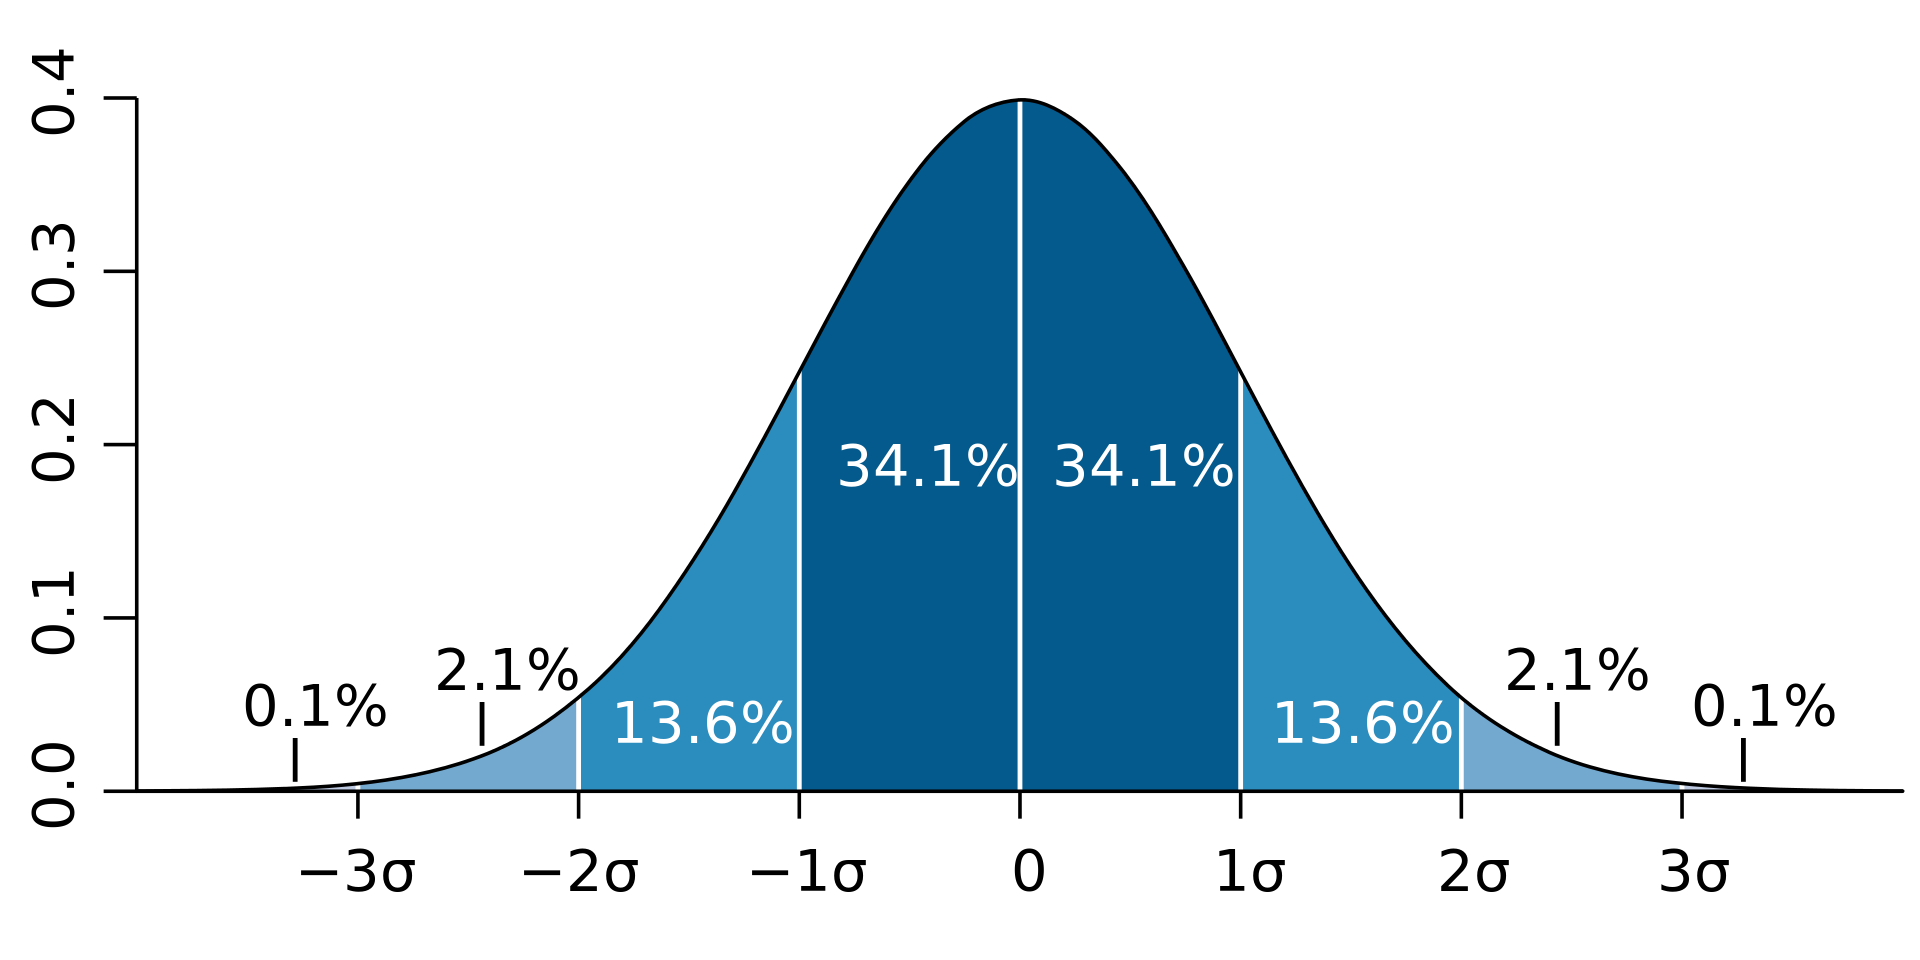
\includegraphics[width=0.5\textwidth]{images/Normalverteilung.png}
    \caption{Intervalle um den Mittelwert einer Normalverteilung \cite{normalverteilung}}
    \label{fig:normalverteilung}
\end{figure}


\subsection{R und RStudio}

\textit{R} ist eine im Jahr 1992 entwickelte Programmiersprache bzw. -umgebung, um statistische Auswertungen und Grafiken zu erzeugen. Sie enthält bereits viele Funktionen zu diesem Zweck, kann aber auch sehr leicht durch Bibliotheken erweitert werden. Auswertungen und Grafiken haben eine entsprechende Qualität, um direkt in Veröffentlichungen genutzt zu werden. Insbesondere für sich wiederholende Auswertungen kann es sehr sinnvoll sein, eigene Skripte mit \textit{R} zu schreiben und diese wiederholt auszuführen. Daten können beispielsweise sehr leicht aus gängigen Datenformaten, wie CSV importiert und verarbeitet werden. Die Sprache hat eine relativ große Bekanntheit und Community, was eine Entwicklung und das Finden von speziellen Lösungen sehr einfach macht. \cite{r}

\textit{RStudio} ist eine für \textit{R} entwickelte Entwicklungsumgebung, die eine einfachere Handhabung möglich macht. Eine grafische Benutzeroberfläche, Syntaxhighlighting, automatische Codeeinrückung o.ä., wie es aus Entwicklungsumgebungen vieler anderer Sprachen bekannt ist, machen die Bedienung sehr viel einfacher, als es noch zum Beginn der Entwicklung von \textit{R} der Fall war. \cite{rstudio}

Für dieses Projekt bietet diese Umgebung eine sehr gute Grundlage zur Auswertung, ohne alle Berechnungen und Zeichnungen manuell anfertigen zu müssen. Es lassen sich sehr systematisch und übersichtlich eine Aufarbeitung der Daten und anschließende Darstellung in Form von Graphen erzeugen, sodass eine einfache Interpretation möglich ist. Es ist sehr unkompliziert, die zuvor beschriebenen mathematischen Methoden auf die Messwerte anzuwenden. Auch wenn diese nicht besonders kompliziert sind, lassen sich so dennoch Fehler vermeiden und Berechnungen für große Datenmengen auf einmal durchführen.
